
\chapter{Clickbaits und die Klassifizierung von Clickbaits}% \chapter{Checkliste}


\section{Einleitung}
Clickbaits besitzen semantische und syntaktische Nuancen, auf die besonders vorgegangen werden muss. Dies geschieht in Form von analyse und vorverarbeitung der Titel. In diesem Abschnitt werden Ansätze aus der Literatur verglichen, die diese semantischen und syntaktischen Besonderheiten bearbeiten. In diesem Kapitel werden Ansätzte aus der Literatur vorgestellt, die die Aufgabe Clickbait Klassifizierung und die damit entstehenden Unteraufgaben wie das Sammeln von Daten, Einbetten der Wörter und schließlich entwickeln der Deep Learning Modelle haben.



\section{Was sind Clickbaits?}
Was sich hinter einer Schlagzeile, einem Titel verbirgt ist ohne weiteres nicht ersichtlich. Die meisten Menschen nehmen heutzutage Ihre Nachrichten über soziale Medien auf. Auf sozialen Medien werden meistens nur die Schlagzeilen gezeigt und wenn der Nutzer einen entsprechenden Eintrag interessant oder lesenswert findet, klickt er auf diesen Link. Das Wort Clickbait stammt aus den beiden Wörtern \enquote{Klick} und \enquote{Köder}, es ist also eine Falle. Viele Medienunternehmen, teilweise auch große, nutzen diese Falle um mehr Klicks zu generieren. Das Problem dabei ist es oftmals, dass die Nutzer durch die \enquote{Spannung} oder \enquote{Frage} in der Schlagzeile eine Erwartung haben, die nicht immer oder nur teilweise erfüllt wird. In der Studie von \cite*{Main} wurden ca. 1,6 Mio. Facebook-Posts untersucht und es wurde festgestellt, dass 25 bis 60\% der Fälle Clickbaits-Posts waren, je nach Medienunternehmen und Thema.

Es gibt keine eindeutige Definition für Clickbaits. Clickbaits weisen unterschiedliche Formen. Nach \cite*{Biyani2016} sind Clickbaits, als eine Praxis um Klicks zu generieren, durch eine attraktive Überschrift, wessen Inhalt die Erwartungen nur teilweise oder gar nicht erfüllt. Clickbaits kann also eine Täuschung oder Trick der Medien betrachtet werden. Eine andere Definition \cite*{Potthasta} betrachtet das Thema Clickbait eher als Werbung für Onlineinhalte und die damit verbundene verbreitung oder viral gehen durch die sozialen Medien.

\begin{figure}[H]
    \centering
    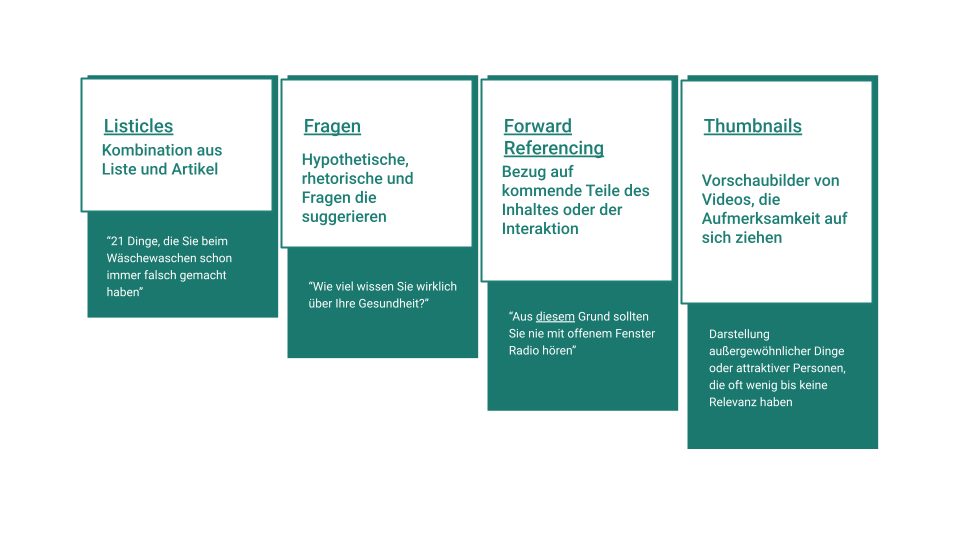
\includegraphics[width=14cm]{kapitel4/clickbaits.png}
    \caption[Die Kernformen des Clickbaits]{Die 4 Kernformen des Clickbaits in Anlehnung an \cite*[71]{Hrsg2020}}
    \label{TSNE}
\end{figure}

In \cite*[70-71]{Hrsg2020} werden CLickbaits formal in 4 Kategorien aufgeteilt. Der Autor bezieht sich dabei auf 4 Quellen und teilt Clickbaits als Listicles \cite*{Vijgen2014}, Fragen \cite*{Lai2014}, Forward Referencing \cite*{Blom2015} und Thumbnails \cite*{Zannettou2018} auf. Diese 4 Kategorien betrachtet der Autor als Kernkategorien. Aus \cite*[71]{Hrsg2020} werden Clickbaits außerdem in weitere Gestaltungsformen wie etwa, dass sie \enquote{Übertreibungen} sein können also falsche Versprechen geben, oder irreführend sind und unklar sein können.Es wird außerdem auf die unangemessene und vulgäre Sprache und der Formatierung, wie etwa den übertriebenen Gebrauch von Großschreibung oder Satzzeichen aufmerksam gemacht. Der Autor macht auf \cite*[75-76]{Hrsg2020} deutlich, dass Clickbaits kein neu eingesetztes Stilmittel im Journalismus sei. Schließlich verwendet der Autor den Begriff \enquote{Neugier} beim Leser. Leser wollen oftmals über Themen wie Tod, Gewalt, Sex und Prominente \cite*{Tenenboim2015} unterhalten werden.




\section{Wie werden Clickbaits klassifiziert?}
Mit der Arbeit aus \cite*{Chakrabortya} wurde eine Browser-Erweiterung erstellt, welches Clickbaits erkennen soll. Es wurden umfangreiche Daten sowohl für Clickbaits als auch für Nicht-Clickbait-Kategorien gesammelt. Für die Nicht-Clickbaits-Kategorien wurden 18.513 Wikinews Artikeln gesammelt. Der Vorteil dieser Artikel ist, dass diese von einer Community erstellt werden und jeder Nachrichtenartikel vor der Veröffentlichung von der Community geprüft werden. Es gibt Stilrichtlinien, die eingehalten werden müssen. Um Clickbaits zu finden, haben die Autoren manuell aus Seiten wie \enquote{Buzzfeed} oder \enquote{Upworthy} ca. 8000 Titel gecrawlt. Um falsche Negative zu vermeiden (d. h. die Artikel in diesen Bereichen, bei denen es sich nicht um Clickbaits handelt), wurden sechs Freiwillige rekrutiert um die Überschriften zu labeln. Schließlich wurden 7500 Titel zu jeder der beiden Kategorien zugefügt.

% \section{Analyse Textdaten}


Laut \cite*{Chakrabortya} sind die herkömmlichen Nicht-Clickbait Schlagzeilen kürzer als Clickbait Schlagzeilen. Traditionelle Schlagzeilen enthalten in der Regel meistens Wörter, die sich auf bestimmte Personen und Orte beziehen, während die Funktionswörter den Lesern zur Interpretation aus dem Kontext überlassen bleiben. Es wird hier als Beispiel gegeben \enquote{Visa-Deal oder kein Migranten-Deal, Türkei warnt EU}. Hier sind die meisten Wörter Inhaltswörter, die die wichtigsten Erkenntnisse aus der Geschichte zusammenfassen, und es gibt nur sehr wenige Verbindungsfunktionswörter zwischen den Inhaltswörtern. Auf der anderen Seite sind Clickbait Schlagzeilen länger. Die Sätze, enthalten sowohl Inhalts- als auch Funktionswörter. Ein Beispiel für solche Schlagzeilen ist \enquote{Ein 22-Jähriger, dessen Ehemann und Baby von einem betrunkenen Fahrer getötet wurden, hat ein Facebook-Plädoyer veröffentlicht}. Obwohl die Anzahl der Wörter in Clickbait-Schlagzeilen höher ist, ist die durchschnittliche Wortlänge kürzer. Es werden häufig Wörter verwendet wie \enquote{Sie werden}, \enquote{Sie sind}. Im Durchschnitt haben die Wörter bei den Clickbaits längere Abhängigkeiten als Nicht-Clickbaits. Der Hauptgrund ist die Existenz komplexerer Phrasensätze im Vergleich zu Schlagzeilen ohne Clickbait. Es ist außerdem zu sehen, dass in Clickbait-Schlagzeilen Stoppwörter häufiger verwendet werden. Clickbait Überschriften verwenden häufig Determinantien wie \enquote{ihre}, \enquote{meine}, die auf bestimmte Personen oder Dinge im Artikel verweisen. Die Verwendung Wörter dient in erster Linie dazu, den Benutzer neugierig auf das Objekt zu machen, auf das verwiesen wird, und ihn zu überzeugen, den Artikel weiter zu verfolgen. Um Daten zu erfassen, können auch Soziale Medien wie Twitter herangezogen werden, wie im Beispiel von \cite*{Potthast}.


% \section{Feature Selection}
Um lexikalischer und semantische und orthografische und morphologische Merkmale zu erfassen, benutzen die Autoren aus \cite*{Anand2019} Worteinbettungen und Zeicheneinbettungen, anstatt übermäßig Feature Selection auszuüben. Um Informationen außerhalb einzelner oder fester Wortfenster zu erfassen, untersuchten die Autoren dabei verschiedene RNN-Architekturen (Recurrent Neural Network) wie LSTM (Long Short Term Memory), GRU (Gated Recurrent Units) und Standard-RNNs. Dieses sind Wiederkehrende neuronale Netzwerkmodelle, die für sequentielle Daten wie Sprache und Text gut modelliert werden können.


Die Arbeit von \cite*{Agrawal2017} schlägt ein Modell vor, welches CNNs benutzt. CNNs werden für verschiedene Deep-Learning-Aufgaben verwendet. Es wurde nur eine Faltungsschicht in das CNN-Modell eingebaut. Die erste Schicht wird für das Einbetten der Wörter in Vektoren verwendet. Dabei wurden 2 verschiedene Worteinbettungen in Bezug genommen. Ein vortrainiertes und eines welches von Grund auf lernen musste und sich während des Trainings weiterentwickelt. In der nächsten Schicht werden Filter in verschiedenen Größen verwendet um Faltungen über Wortvektoren zu erzeugen.

Die Autoren der Arbeit aus \cite*{Pujahari} Clustern zunächst die aus den Schlagzeilen erstellten Vektoren mit der sogenannten t-SNE Methode nach \cite{VanDerMaaten2008}. Dieser Algorithmus \enquote{rekategorisiert} die Schlagzeilen in mehrere Gruppen und reduziert die vielen Dimensionen von Clickbaits im Datensatz. Die Autoren beginnen erst im nächsten Schritt mit dem Training. Dabei entstehen 11 Kategorien von Clickbaits (Mehrdeutig, Übertreibung oder Neckerei).


\begin{figure}[H]
    \centering
    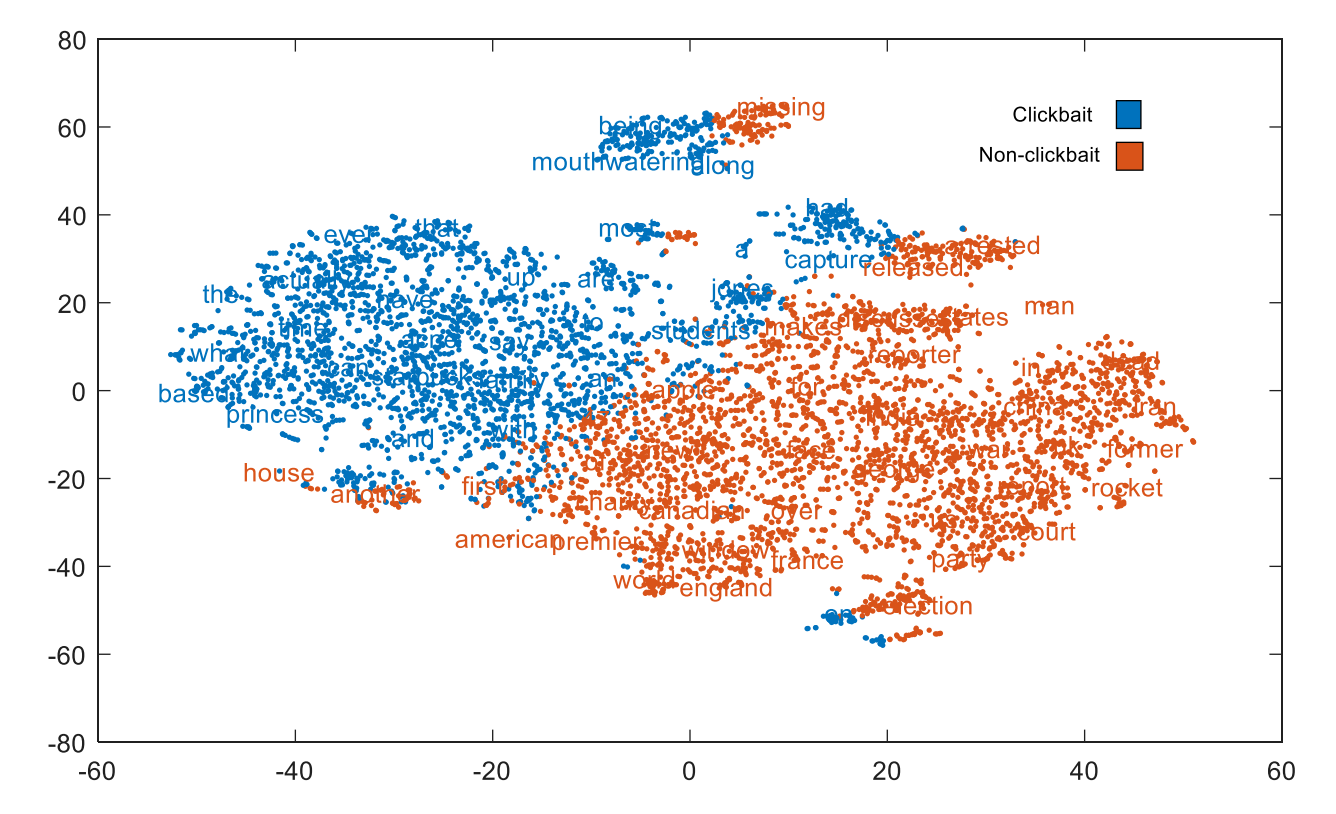
\includegraphics[width=12cm]{kapitel4/tsne.png}
    \caption[Clustering von Überschriften mit t-SNE]{Die Autoren verwenden das t-SNE Algorithmus nach \cite{VanDerMaaten2008} um die Dimensionen zu Reduzieren und es entstehen mehrere Unterkategorien von Clickbaits. Entnommen aus \cite*{Pujahari}.}
    \label{TSNE}
\end{figure}

\section{Schluss}
In diesem Kapitel wurden einige Arbeiten aus der Literatur vorgestellt, jedoch nicht alle. Es gibt außerdem noch weitere Arbeiten wie \cite*{chawda2019novel}\cite*{Zannettou2018}\cite*{Kumar}\cite*{Thomas}\cite*{Liao}\cite*{Glenski} und \cite*{Biyani2016} die unter diese Literaturstudie fallen könnten. Alle diese Arbeiten in Ihrer ganzen Fülle zu beschreiben würde den Rahmen dieser Arbeit sprengen, sodass nur ein Einblick über mögliche Aufgaben, wie das Sammeln von Daten und das Bauen eines Deep Learning Ansatzes sowie die Besonderheiten die Clickbaits Schlagzeilen haben, verschafft wurde.
